\documentclass{scrartcl}

\usepackage{helvet}
\usepackage[T1]{fontenc}
\usepackage[ngerman]{babel}
\usepackage[utf8]{inputenc}
\usepackage{enumitem}
\usepackage{hyperref}
\usepackage{graphicx}
\usepackage{cleveref}
\usepackage[autostyle=true,german=quotes]{csquotes}
\renewcommand{\familydefault}{\sfdefault}
%----------------------------------
% thomi fa list implementation
%----------------------------------

\newlist{falist}{enumerate}{2}
\setlist[falist,1]{label={/FA\arabic{falisti}\arabic{falistii}/},align=left,labelwidth=17pt,labelsep=3pt,leftmargin=20pt}
\setlist[falist,2]{label={/FA\arabic{falisti}\arabic{falistii}/}}%,align=left,labelwidth=17pt,labelsep=3pt,leftmargin=0pt}

\usepackage{chngcntr}
\counterwithin{falistii}{falisti}

\newlist{pdlist}{enumerate}{2}
\setlist[pdlist,1]{label={/PD\arabic{pdlisti}\arabic{pdlistii}/},align=left,labelwidth=17pt,labelsep=3pt,leftmargin=20pt}
\setlist[pdlist,2]{label={/PD\arabic{pdlisti}\arabic{pdlistii}/}}%,align=left,labelwidth=17pt,labelsep=3pt,leftmargin=0pt}
\counterwithin{pdlistii}{pdlisti}

\newlist{nflist}{enumerate}{2}
\setlist[nflist,1]{label={/NF\arabic{nflisti}\arabic{nflistii}/},align=left,labelwidth=17pt,labelsep=3pt,leftmargin=20pt}
\setlist[nflist,2]{label={/NF\arabic{nflisti}\arabic{nflistii}/}}%,align=left,labelwidth=17pt,labelsep=3pt,leftmargin=0pt}
\counterwithin{nflistii}{nflisti}

\newlist{telist}{enumerate}{2}
\setlist[telist,1]{label={/T\arabic{telisti}\arabic{telistii}/},align=left,labelwidth=17pt,labelsep=3pt,leftmargin=20pt}
\setlist[telist,2]{label={/T\arabic{telisti}\arabic{telistii}/}}%,align=left,labelwidth=17pt,labelsep=3pt,leftmargin=0pt}
\counterwithin{telistii}{telisti}

\begin{document}


\title{Pflichtenheft: Lambda - Das Spiel, \\ Die Entwickler}
\author{Luca Becker, Henrike Hardt,\\Larissa Schmid, Adrian Schulte,\\Maik Wiesner}
\date{\today}
\maketitle

\includegraphics[width=\textwidth]{assets/Lambdolino}
\thispagestyle{empty}

\clearpage

\thispagestyle{empty}
\tableofcontents
\thispagestyle{empty}

\clearpage
\setcounter{page}{1}






% ---------------
% Einleitung
% ---------------

\section{Einleitung}

Der derzeitige und auch kommende Ingenieursmangel in Deutschland ist
schon seit Langem Thema in den Medien. „Auf jeden Bewerber kommen
etwa 4 freie Stellen“%
\footnote{http://www.ingenieurwesen-studieeren.de/ingenieurmangel/, aufgerufen am 04.11.14%
}, „jeder zweite angehende Ingenieur bricht sein Studium ab“%
\footnote{http://www.zeit.de/studium/hochschule/2013-10/ingenieure-unis-fachkraeftemangel, aufgerufen am 04.11.14%
}, all diese Nachrichten geben Grund zur Sorge in Hinblick auf Deutschland
als Technologiestandort. Unsere Volkswirtschaft beruht nicht mehr
auf Wertschöpfung aus dem ersten und zweiten, sondern vor allem aus
dem dritten Sektor – damit dies weiterhin funktionieren kann, werden
vor allem Ingenieure benötigt. Doch an dem derzeitigen Mangel ist
nicht nur die Überalterung unserer Gesellschaft schuld, sondern vor
allem auch die fehlende Begeisterung von Jugendlichen für die sogenannten
MINT-Fächer (Mathematik, Informatik, Naturwissenschaft, Technik).
Um Deutschland als Standort auch weiterhin wettbewerbsfähig zu halten,
ist es somit wichtig, Kinder schon frühestmöglich spielerisch an Fragestellungen
aus diesen Bereichen heranzuführen. 

In der Informatik ist der Lambda-Kalkül ein wichtiges Konstrukt, der
zum Beispiel die Entwicklung funktionaler Programmiersprachen wesentlich
beeinflusst hat. Obwohl er damit eine große Bedeutung hat und sehr
mächtig ist in Bezug auf sowohl die Theoretische Informatik als auch
funktionale Programmierung, so sind die grundlegenden Regeln dennoch
nicht allzu komplex und leicht verständlich. 

Um Kindern also schon im Grundschulalter eine erste Auseinandersetzung
mit Themen der Informatik und damit auch der Ingenieurswissenschaften
zu bieten, eignet sich der Kalkül also sehr gut. Unsere nachfolgend
dargelegte Visualisierung der Funktionsweise des Kalküls mithilfe
von einfachen Formen und sie ineinander umwandelnden Maschinen ist
dabei besonders kindgerecht, wodurch der Kalkül anhand von einfachen
Lambda-Ausdrücken einfacher verstanden und verinnerlicht werden kann.
Diese Idee soll nun als Android-App umgesetzt werden, sodass Kinder
selbständig spielen können, der Fortschritt im Spiel aber auch jederzeit
durch Eltern oder Lehrkräfte einsehbar ist. 

\clearpage








% ---------------
% Zielbestimmungen
% ---------------

\section{Zielbestimmungen}


Die Kinder sollen durch das Spiel in die Lage versetzt werden, sich die Prinzipien des Lambda Kalküls spielerisch zu erarbeiten ohne über Vorkenntnisse zu verfügen.

\subsection{Musskriterien}

\begin{enumerate}
	\item \label{muss:vermittelnlamba}Spielerisches Vermitteln des Lambda Kalküls für Kinder ab acht Jahren
	\item \label{muss:simulationandroid}Das Spiel muss in der Simulationsumgebung von Android laufen
	\item \label{muss:touchinterface}komplett über das simulierte Touchinterface bedienbar sein
	\item \label{muss:mvc}eine modulare Architektur besitzen (z.B. Model-View-Controller-Prinzip)
	\item \label{muss:5indilevel}mindestens fünf individuelle Level
	\item \label{muss:tutorial}Tutorial Level
\end{enumerate}

\subsection{Wunschkriterien}

\begin{enumerate}
	\item \label{wunsch:werkstatt}Werkstatt zum Umbauen von Maschinen
	\item \label{wunsch:highscore}Highscore-Tabelle
	\item \label{wunsch:challengemode}Challengemode mit Zeitdruck
	\item \label{wunsch:multilang}Auslieferung in mehreren Sprachen
	\item \label{wunsch:8bit}Pixelgrafik / Retroloook / reduzierter Farbraum
	\item \label{wunsch:multiplechar}Mehrere Spielcharaktere (männlich, weiblich)
	\item \label{wunsch:multiplemode}Mehrere Spielmodi (siehe Aufgabentyp \ref{aufgabentyp:fehlerfindung})
    \item \label{wunsch:story}Begleitende Story %link zu eintrag
    \item \label{wunsch:erweiterndeLevelelemente}Erweiternde Levelelement, z.B. Leitern, Aufzüge usw.
\end{enumerate}

\subsection{Abgrenzungskritieren}

\begin{enumerate}
	\item \label{abgrenz:online}Kein Onlinemodus
	\item \label{abgrenz:multiplayer}Kein Multiplayer Modus
	\item \label{abgrenz:emu}Keine vorgesehene Kompatiblität mit anderen Geräten/Betriebssystem ohne Emulation
\end{enumerate}

\clearpage










% ---------------
% Spielaufbau
% ---------------

\section{Spielaufbau}

\subsection{Spielprinzip}
Das Spielprinzip beruht auf dem Bewegen von Blöcken, indem der Spieler die Blöcke hochhebt und wieder absetzt. Der Spieler muss die verschiedenen Teile des Spieles, die Maschinen(), die Maschinen-Cluster() und die Metallstücke, in die dafür vorgesehenen Positionen bringen. Hat er alle Teile in die richtigen Positionen gebracht, öffnet sich die Tür zum nächsten Level.


\subsection{Spielelemente}

Zu Beginn eines Levels wird die Spielerfigur angezeigt und bewegt zweidimensional durch die Welt und wird vom Spieler gesteuert.

\begin{description}
	\item[Spielerfigur] bewegt sich durch die Welt, sammelt Gegenstände um mit diesen die Levelquest zu lösen
	\item[Leben] Jeder Spieler hat je Level drei Leben, die er verlieren kann, wenn er ins Wasser fällt
	\item[Spielwelt] zweidimensionale Spielwelt auf einem Raster basierend, in der sich der Spieler bewegt
	\item[Spielebenen] verschiedene Ebenen in der Spielwelt auf die der Spieler springen kann, sie sind auf einem Raster angeordnet
		\begin{enumerate}[label=\arabic*]
			\item Landebenen: Auf diesen Ebenen liegen die Collectable Items
			\item Wasserebenen: Fällt der Spieler in das Wasser, muss er wieder am linken unteren Rand anfangen und er verliert ein Leben, hat er kein Leben mehr, so muss er das Level neu beginnen
		\end{enumerate}
	\item[Collectable Items] \label{elemente:collectable}sind in der Spielwelt verteilt und müssen von der Spielfigur eingesammelt werden um im Rätselteil eingesetzt zu werden. Diese bestehen aus:
	\begin{enumerate}[label=\arabic*]
		\item Maschinen (entspricht der Abstraktion)
		\item Metallstücke (entspricht der Variablen)
		\item Maschinen-Cluster (entspricht der Applikation)
	\end{enumerate}
	\item[Levelquest] sind gegebene Aufgaben die zum Abschließen des Levels erfüllt werden müssen
	\item[Leveltür] bildet den Abschluss eines Levels. Sobald alle Quests in dem Level gelöst wurden wird die Tür freigeschaltet
\end{description}

\subsection{Regeln}

\begin{description}

\begin{minipage}{1\textwidth}
	\item[Spielregeln] \label{spielaufbau:Spielregeln} Die Spielfigur beginnt an der unteren, linken Ecke der Spielwelt und muss es schaffen die Tür an der rechten unteren Ecke zu öffnen. Dies gelingt ihm in dem er diverse Objekte (Maschinen, Metallobjekte und Maschinen-Cluster)auf dem Spielfeld in Position bringt, sodass diese nach den Prinzipien des Lambda Kalküls einen Lambdaausdruck bilden  welcher zu einem gewünschten Ergebnis zusammengefasst oder gelöst werden kann.\\
	Der Spieler muss neben einem Objekt stehen, um dieses aufheben zu können.\\
	Der Spieler kann immer nur ein Objekt tragen. Um ein anderes Objekt aufzuheben muss er erst das Objekt das er trägt ablegen.\\
	Um auf die oberen Ebenen der Spielwelt zu gelangen, kann die Spielfigur springen, dabei ist zu beachten, dass die Figur nur eine feste Höhe hochspringen kann und er somit auf Ebenen außerhalb seiner Reichweite, nicht durch einfaches Springen gelangen kann. Die Figur kann auch springen wenn sie etwas in den Händen trägt (dabei kann es zu einer geringen Trägheit kommen, z.B. ungenauere Spielsteuerung(diese ist gewollt und soll das Spiel ein wenig schwieriger gestalten)).\\
	Befindet sich in jedem freien Feld ein Objekt, wird der daraus resultierende Lambdaausdruck ausgewertet. Falls die Maschinen und Metallstücke an den richtigen Positionen stehen und der $\lambda$-Kalkül erfüllt ist, wird dem Spieler das Ergebnis und die spezifische Abarbeitung des Maschinenkonstrukts nach den regeln des $\lambda$-Kalküls gezeigt. Anschließend öffnet sich die Tür am Level ende und das Level gilt als geschafft sobald diese erreicht ist.\\
	
\end{minipage}

\begin{minipage}{1\textwidth}
	\item[Die Verarbeitungsregel der Maschinen] Die Verarbeitung der einzelnen Metallstücke erfolgt in fester Reihenfolge.\\
	Es wird immer nur ein Metallstück zu einem bestimmten Zeitpunkt verarbeitet.\\
	Wie das Objekt verarbeitet wird bestimmt die jeweilige Maschine.\\
	Was die Maschine verarbeiten soll befindet sich immer rechts neben dieser Maschine.\\
	Die Maschinen werden in fester Reihenfolge angeordnet und verarbeiten nacheinander die gegebenen Metallobjekte.\\
	Dabei kann jede Maschine nur ein Objekt verarbeiten, nachdem sie dieses Objekt verarbeitet hat verschwindet sie.\\
	Jede Maschine kann die Anzahl des zu verarbeitenden Objekts und ggf. dessen Farbe/Muster verändern. Hierbei ist zu beachten das eine Maschine auch ein Objekt komplett entfernen kann. Was eine Maschine genau am zu verarbeitenden Objekt verändert ist durch ihr aussehen eindeutig bestimmt.\\
	Das verarbeitete Objekt landet im Bereich unterhalb der Maschine an vorgegebenen Stellen.\\
	Nachdem die Maschine verschwunden ist rücken die Objekte unter ihr alle um eine Position nach oben, und die in der obersten Ebene am weitesten links liegende Maschine beginnt die Verarbeitung.\\
\end{minipage}	
	
\begin{minipage}{1\textwidth}
	\item[Sonderfälle/regeln:] Maschinencluster: Ein Maschinencluster ist eine besonderer Form der Maschinen, sie verarbeitet keinen Input sondern dient als eine Art \enquote{Klammerung}. Ist ein Maschinencluster an der Reihe zu arbeiten, so verarbeitet sie keinen Input. Stattdessen werden alle Objekte in diesem Cluster nach den normalen Verarbeitungsregeln zuerst verarbeitet, bis nur noch eine Maschine und eine Menge an Metallobjekten darin vorhanden sind. Danach verschwindet der Cluster und sein Inhalt übernimmt seinen Platz in der aktuellen Verarbeitung.\\
\end{minipage}

\end{description}

\subsection{Aufgabentypen}
In jedem Spieltyp läuft im Hintergrund ein Timer mit, der die Spielzeit des Levels misst. Dadurch können Timer-Achievements freigeschaltet werden.
\begin{enumerate}
	\item \label{aufgabentyp:puzzle} Puzzle: Aufgabentyp bei dem an die vorgegebenen stellen Maschinen, Metallobjekte oder Maschinen-Cluster eingefügt werden müssen um einen $\lambda$-Ausdruck zu bauen der ein gewünschtes Ergebnis liefert oder einen gewünschten Endzustand hat.\\
	Die benötigten Teile sind in der Spielwelt verstreut und müssen an den passenden Stellen eingefügt werden.\\
	Der Spieler kann dabei immer nur ein Objekt tragen.\\
	Es sind auch falsche Konstellationen möglich die zu einem falschen Ergebnis führen.\\
	\item \label{aufgabentyp:fehlerfindung} Fehlerfindung: Aufgabentyp bei dem der $\lambda$-Ausdruck schon fertig zusammengesetzt ist, jedoch nicht in der richtigen Konstellation.\\
	Der Spieler muss die Fehler finden und die entsprechenden Objekte austauschen.\\
	\item \label{aufgabentyp:ergebnis} Ergebnisbestimmung: Die Maschinenkonstruktion ist gegeben, der Spieler muss mit einer gegebenen Menge an Elementen die Endkonstellation bestimmen und angeben. ($\beta$ - Reduktion durchführen) 
\end{enumerate}

\clearpage







% ---------------
% Produkteinsatz Anforderungen
% ---------------


\section{Produkteinsatz}

Das Produkt soll auf jedem Android Gerät ab Android 4.2 einsatzfähig sein. Ein Einsatz auf Emulatoren der Android Plattform ist ebenfalls vorgesehen.

\subsection{Anwendungsbereich}

\begin{enumerate}
	\item Freizeitgestaltung von Kindern ab 8 Jahren
	\item Einsatz an Vor- und Grundschulen
\end{enumerate}

\subsection{Zielgruppen}

Die Zielgruppe besteht überwiegend aus Kindern im Alter von acht bis zwölf Jahren, die das Spiel entweder aus Interesse oder im Rahmen eines Projektes an der Schule spielen. Hierbei wird ihnen subtil der Umgang mit dem $\lambda$-Kalkül beigebracht.

\clearpage







% ---------------
% Produktumgebung
% ---------------

\section{Produktumgebung}

\subsection{Software}

\begin{itemize}
	\item Die Software ist für die Unterstützung der API 17+ (Android 4.2) von Android ausgelegt
\end{itemize}

\subsection{Hardware}

\begin{itemize}
	\item Die eingesetzte Hardware muss über ein Touch-Interface verfügen.
	\item Das Spiel ist für die Verwendung mit einem Tablet-Gerät ausgelegt.
	\item Eine Verwendung mit einem Smartphone soll jedoch auch möglich sein.
\end{itemize}

\clearpage








% ---------------
% Funktionale Anforderungen
% ---------------

\section{Funktionale Anforderungen}

\begin{falist}
	\item \label{fa:tutorial}Tutorial Modus (Musskriterium \ref{muss:tutorial}) findet nach dem ersten Starten des Spiels statt
	\begin{falist} 
        \item \label{fa:tutorial_01}Der Tutorial Modus basiert auf einem Minimum an textuellen Erklärungen
        \item \label{fa:tutorial_02}Erklärt die Funktionsweise des Spiels
		\item \label{fa:tutorial_03}Ein wiederholtes Starten des Tutorial Modus ist möglich
	\end{falist}
	\item \label{fa:spielerprofile} Spielerprofile
	\begin{falist}
		\item \label{fa:spielerprofile_anlegen} Anlegen von Spielerprofilen
		\item \label{fa:spielerprofile_bearbeiten} Bearbeiten von Spielerprofilen
		\item \label{fa:spielerprofile_loeschen} Löschen von Spielerprofilen
		\item \label{fa:spielerprofile_wechseln} Wechseln zu Spielerprofilen
	\end{falist}
	\item \label{fa:levelmenue}Levelmenü bietet eine Übersicht über alle Level des Spiels (Musskriterium \ref{muss:5indilevel}). Diese sind unterteilt in abgeschlossene und nicht abgeschlossene Level.
    \begin{falist}
        \item Das erste Level ist automatisch freigeschaltet
        \item Die restlichen Level werden durch das Beenden des vorherigen Levels freigeschaltet
    \end{falist}
    \item \label{fa:spielen} Level spielen
	\item \label{fa:spieleinstellungen} Spieleinstellungen
	\item \label{fa:spielestatistiken} Spielestatistiken
	\item Interaktion mit den Spielelementen aus Nr. \ref{elemente:collectable}
	\begin{falist}
		\item Aufnehmen von Spielelementen
		\item Abgabe für die Levelquests
	\end{falist}
	\item Infobereich, der weiterführende Informationen zum Thema $\lambda$-Kalkül enthält
    \item Achievements, unter anderem
    \begin{falist}
    	\item Abschließen des Tutorial-Modus
    	\item Abschließen eines Kapitels
    	\item Spielzeit unterhalb einer gegebenen Schranke
    	\item Spielzeit oberhalb einer gegebenen Schranke
    	\item Fun-Achievements (Nicht-Schwimmer, Nachtsschwärmer)
    	\item First-Try
    \end{falist}
    \item Animierte Auswertung der Maschinenkonstellation
\end{falist}

\clearpage








% ---------------
% Produktdaten
% ---------------

\section{Produktdaten}
Das Produkt muss Daten speichern und verwalten, insbesondere: 

\subsection{Profildaten}

\begin{pdlist}
    \item Profile, bestehend aus 
    \begin{pdlist}
        \item Name des Spielers
        \item Avatar
        \item profilbezogene Einstellungen(Hintergrund, Musik etc.) 
        \item profilbezogener Spielfortschritt(gelöste Level, Achievements, etc.)
    \end{pdlist}
    \item \label{produktdaten:spielestatistiken} Spielstatistiken
    \begin{pdlist}
        \item Spieldauer
        \item Anzahl gelöste Level
        \item Anzahl Achievements
    \end{pdlist}
\end{pdlist}

\subsection{Einstellungen}
\label{produktdaten:einstellungen}

\begin{pdlist}[resume]
	\item Einstellen der Lautstärke
	\item An/Aus für Lautstärke
\end{pdlist}

\clearpage








% ---------------
% Nichtfunktionale Anforderungen
% ---------------

\section{Nichtfunktionale Anforderungen}

\subsection{Allgemeine Ziele}

\begin{nflist}
    \item Die Navigation durch das Spiel ist für den Spieler intuitiv, unabhängig von seinem Alter
    \item Das Spiel ist insgesamt kindgerecht entworfen, d.h
    \begin{itemize}
    \item Weitestgehend werden Piktogramme verwendet
    \item Textuelle Erklärung (insbesondere das $\lambda$-Symbol) wird nach Möglichkeit vermieden. Falls Text nötig ist, wird einfache, kindgerechte Sprache verwendet
    \end{itemize}
\end{nflist}

\subsection{Benutzbarkeit, Performance, Stabilität}
\begin{nflist}[resume]
	\item Das Starten eines Levels beträgt höchstens 10s 
	\item Das Programm läuft stabil: 
	\begin{nflist}
		\item Es treten keine Abstürze der Software auf 
		\item Ladezeiten befinden sich in einem akzeptablen Rahmen. 
	\end{nflist}
	\item Die Auswertung eines Levels(Sieg oder Niederlage) dauert max. 5 Sekunden. 
	\item mind. 75\% Testüberdeckung 
	\item Es wird nur die Berechtigung für den Speicherzugriff(Lesen
	und Schreiben) benötigt. 
	\item Der benötigte Speicherverbrauch reduziert sich auf ein Minimum. 
	\item Nach Beendigung eines Levels wird der Spielstand automatisch gespeichert.
\end{nflist}

\subsection{Qualität und Rechtliches}

\begin{nflist}[resume]
	\item Das Programm verwendet für Dateien folgende Standards: 
	\begin{itemize}
		\item WAV, OGG, MP3 für Audio Dateien 
		\item SVG für Vektorgrafiken 
		\item PNG, JPG für pixelbasierte Grafiken 
		\item JSON für strukturierte Textdateien.
	\end{itemize}
	\item Die Auslieferung der finalen Version erfolgt in Form einer .apk-Datei.
	\item Impressum und ausschließliche Verwendung von frei verfügbare Bibliotheken
	für den Fall der Veröffentlichung
\end{nflist}

\clearpage







% -------------------------
% Globale Testfälle
%-------------------------

\section{Globale Testfälle}

\subsection{Funktionssequenzen}

\begin{telist}
	\item Tutorial basierend auf \ref{fa:tutorial} - \ref{fa:tutorial_03}
	\begin{itemize}
		\item Der Anwender startet den Tutorial-Modus über das Level-Menü (Systemmodell \ref{appaufbau:Levelauswahl}) oder gelangt automatisch in diesen beim ersten Starten des Spiels mit einem neuen Profil.
		\item Der Anwender wird durch die Tutorial-Level geleitet, in denen ihm erklärt wird, wie er die Steuerung benutzen, die Elemente an die gewünschte Position bringen kann und wie genau die Maschinen die Elemente verarbeiten.
	\end{itemize}

	\item Ein Benutzerprofil anlegen (\ref{fa:spielerprofile_anlegen})
	\begin{itemize}
		\item Der Anwender befindet sich im Einstellungsmenü und drückt auf den \enquote{Benutzerverwaltungsbutton}. Diese Aktion führt den Benutzer zu einer neuen Anzeige, die seine bisherigen Profile beinhaltet.
		\item Durch Wischgesten gelangt der Benutzer an das Ende der Liste, wo sich ein \enquote{+}-Zeichen befindet. Durch Drücken dieses Symbols wird ein neuer Dialog gestartet.
		\item In diesem Dialogfenster kann der Benutzer einen neuen Profilnamen angeben. Durch drücken des \enquote{Weiter}-Buttons gelangt der zu einem weiteren Dialog.
		\item In diesem Dialog kann er einen Charakter auswählen und sowie auswählen, ob dieses Profil im Rechts- oder Linkshänder Modus gespielt werden soll. Der Dialog wird durch Betätigen des \enquote{OK}-Buttons beendet.
	\end{itemize}
	\item Ein Benutzerprofil auswählen (\ref{fa:spielerprofile_wechseln})
	\begin{itemize}
		\item Der Anwender befindet sich im Einstellungsmenü und drückt auf den \enquote{Benutzerverwaltungsbutton}. Diese Aktion führt den Benutzer zu einer neuen Anzeige, die seine bisherigen Profile beinhaltet.
		\item Durch Scrollen kann der Benutzer seine Profile einsehen. Bei Erreichen des gewünschten Profils wählt er dieses durch Berühren aus.
	\end{itemize}
	\item Ein Benutzerprofil löschen (\ref{fa:spielerprofile_loeschen})
	\begin{itemize}
		\item Der Anwender befindet sich im Einstellungsmenü und drückt auf den \enquote{Benutzerverwaltungsbutton}. Diese Aktion führt den Benutzer zu einer neuen Anzeige, die seine bisherigen Profile beinhaltet.
		\item Durch Scrollen kann der Anwender seine Profile einsehen. Er wählt dieses durch Berühren aus. 
	\end{itemize}
	\item Ein Benutzerprofil bearbeiten (\ref{fa:spielerprofile_bearbeiten})
	\begin{itemize}
		\item Der Anwender befindet sich im Einstellungsmenü und drückt auf den \enquote{Benutzerverwaltungsbutton}. Diese Aktion führt den Benutzer zu einer neuen Anzeige, die seine bisherigen Profile beinhaltet.
		\item Der Anwender wählt den \enquote{Bearbeitungs-Button} neben dem Profil, welches er bearbeiten möchte, aus.
		\item Im Bearbeitungsbereich kann der Anwender den Namen, den Avatar und die Steuerungseinstellung (Rechts- oder Linkshänder) verändern.
	\end{itemize}
	\item Level-Menü (\ref{fa:levelmenue})
	\begin{itemize}
		\item Der Anwender kann nur jene Level öffnen, die bereits freigeschaltet wurden, die anderen Level sind sichtbar, aber sie können nicht ausgewählt werden.
	\end{itemize}
	\item Level spielen (\ref{fa:spielen})
	\begin{itemize}
		\item Die Figur reagiert korrekt auf die Steuerung.
		\item Die Steuerung befindet sich auf der Seite, die der Anwender im Profil ausgewählt hat (\ref{szenarien:ProfilBearbeiten}).
		\item Die alle Elemente, die für das Lösen des Levels benötigt werden, sind vorhanden.
		\item Die Elemente sind alle für die Figur erreichbar.
		\item Die Positionen für die Elemente sind vorhanden.
		\item Die Tür öffnet sich wenn alle Elemente korrekt platziert sind.
	\end{itemize}
	\item Spieleinstellungen (\ref{produktdaten:einstellungen})
	\begin{itemize}
		\item Der Anwender kann die Lautstärke verändern. Die Hintergrundmusik wird dem entsprechend lauter oder leiser.
		\item Der Anwender kann wählen, ob die Musik an oder aus sein soll.
	\end{itemize}
	\item Spielestatistiken (\ref{produktdaten:spielestatistiken})
	\begin{itemize}
		\item Der Anwender kann in den Spielestatistiken sehen, wie lange er gespielt, wie viele Level er gelöst und welche Achievements er bereits erreicht hat.
	\end{itemize}
	\item Speicher / Laden von Applikationszustandes
	\item Speichern / Laden von Spielzuständen
\end{telist}

\subsection{Datenkonsistenz}

\begin{telist}[resume]
	\item Der Spielfortschritt eines jeden Profils wird unabhängig von den anderen Profilen gespeichert und verwaltet. Im Spielfortschritt eingeschlossen sind die Achievements des jeweiligen Nutzers.
	\item Das Anlegen zweier Profile, die über den selben Namen verügen, ist nicht gestattet. Sollte der Benutzer sich dazu entschließen ein Profil zu löschen, wird der Name wieder freigegeben und kann für ein neues Profil verwendet werden.
\end{telist}

\clearpage











% ---------------
% Systemmodelle
% ---------------
\section{Systemmodelle}

\subsection{Allgemeine Appaufteilung}

Der hier gezeigte Systemaufbau ist lediglich eine grobe \enquote{Skizze},
die die zusammenhänge zwischen den einzelnen Menüs sowie, 
die Gestaltung und Aufteilung der App verdeutlichen soll.\\
Allgemein gilt jedoch, das so viel wie möglich ohne Text, sondern durch Symbolik erklärt bzw. dargestellt werden soll. Da die Zielgruppe nicht zwangsläufig lesen und schreiben kann.\\

\begin{enumerate}
	\begin{minipage}{1\textwidth}
		\item \subsection*{Ladebildschirm:} \label{appaufbau:Ladebildschirm}
		Nach dem Starten der App, öffnet diese im Ladebildschirm, hier werden für die App notwendige Daten geladen, um zu Garantieren das das Spiel flüssig und Fehlerfrei läuft. Benutzeingaben sind zu diesem Zeitpunkt nicht möglich.\\
		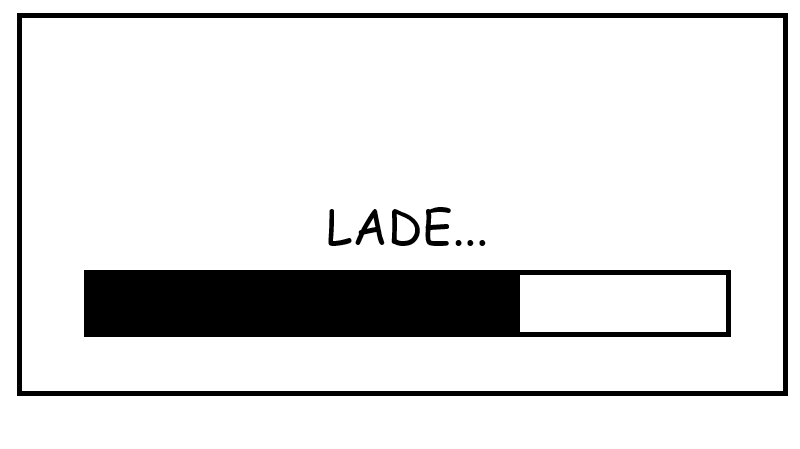
\includegraphics[width=\textwidth]{assets/LoadScreen}
	\end{minipage}
	
	\begin{minipage}{1\textwidth}
		
		\item \subsection*{Profilmenü:}
		Das Profilmenü öffnet sich unmittelbar nach erfolgreicher Beendigung des Ladevorgangs(Nähere Informationen zum Ablauf und Ausnahmen folgen im Kapitel Szenarien).\\
		Die einzelenn Spielerprofile werden durch anzeige des Avatar / Spielecharakters sowie den zugehörigen Profilnamen bestimmt.\\
		Es gibt eine maximale Anzahl an Spielerprofilen, sollte diese erreicht sein so verschwindet der Button zum erzeugen eines neuen Profils.\\
		Gleichzeitig muss immer ein Spielerprofil vorhanden sein, sollte es nur noch ein Spielerprofil geben , so kann dieses nicht gelöscht werden , bis ein weiteres Profil angelegt wurde.\\
		In diesem Menü kann der Spieler aus den bestehenden Spielerprofilen auswählen oder in das Menü zum anlegen eines neuen Spielers gelangen.\\
		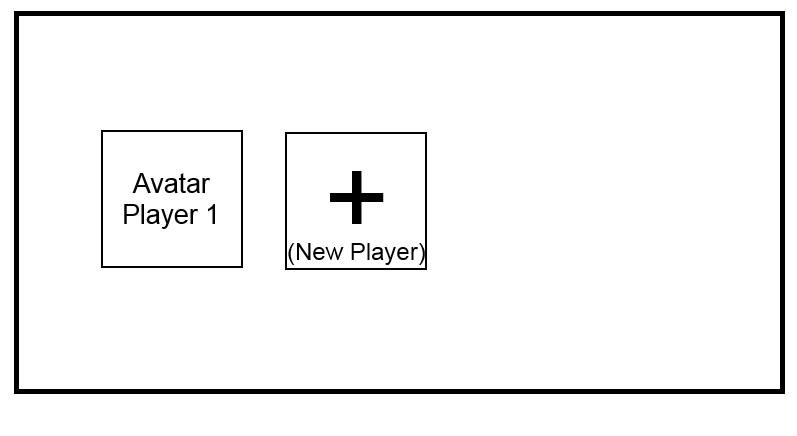
\includegraphics[width=\textwidth]{assets/PlayerScreen}
	\end{minipage}
	
	\begin{minipage}{1\textwidth}
		\item \subsection*{Profil anlegen:}
		In diesem Menü kann ein neues Spielerprofil vom Spieler angelegt werden.\\
		Der Spieler kann einen Namen für das Profil eingeben und aus einer gegebenen Menge an Avataren bzw. Avatarteilen einen als Identifikationsmerkmal aussuchen bzw zusammen setzen.\\
		Der gewählte Avatar dient im weiteren Verlauf auch als Spielfigur, wobei jedoch keine Unterschiede außer dem aussehen zwischen den einzelnen Figuren besteht(Alle sind gleich groß, schnell...).\\
		Auch die Wahl ob man als Linkshänder oder Rechtshänder spielen will kann hier Profil spezifisch gewählt werden.\\
		Man kann jederzeit über das Einstellungsmenü hierhin gelangen um Änderungen am Profil vorzunehmen.\\
		Sollte der Spieler hier abbrechen, so gelangt er zurück ins Profilmenü, ansonsten landet er entweder im Tutorial oder im Hauptmenü(Mehr dazu im Kapitel Szenarien)\\
		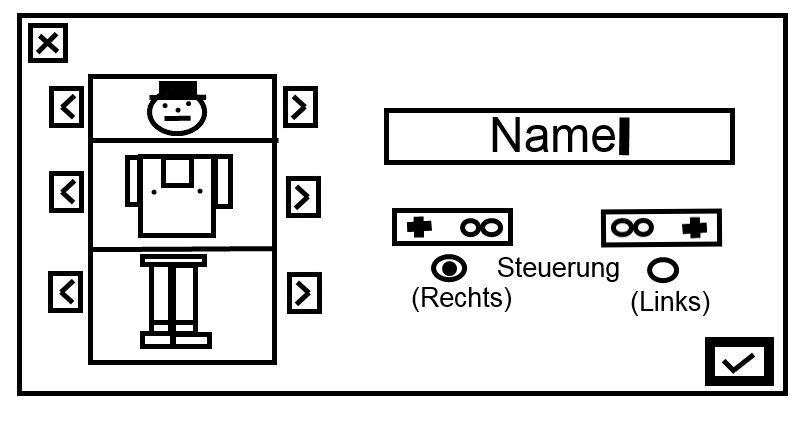
\includegraphics[width=\textwidth]{assets/CreateProfile2}
	\end{minipage}
	
	\begin{minipage}{1\textwidth}
		\item \subsection*{Hauptmenü:} \label{appaufbau:Hauptmenü}
		Dies ist der Zentrale Knotenpunkt der App.\\
		Von hier aus kann der Spieler zur Stageauswahl, den Einstellungen, seiner Statistik, zurück ins Profilmenü gelangen oder das Spiel komplett verlassen.\\
		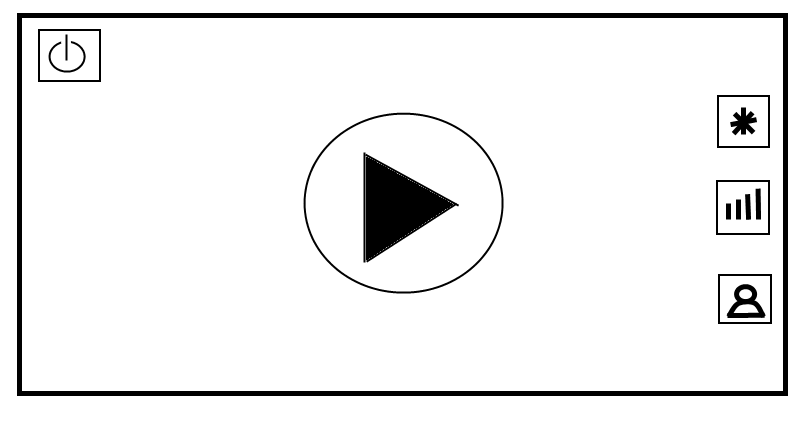
\includegraphics[width=\textwidth]{assets/Mainmenu}
	\end{minipage}
	
	\begin{minipage}{1\textwidth}
		\item \subsection*{Einstellungen:}
		Hier können verschiedene grundlegende Einstellungen vorgenommen werden.\\
		Von hier gelangt man ins Profilbearbeitungsmenü und zur Ansicht aller Achievments (Achievmentmenu).\\
		Der Zurück-Button führt ins Hauptmenü, beim verlassen werden sämtliche Änderungen automatisch gespeichert.\\
		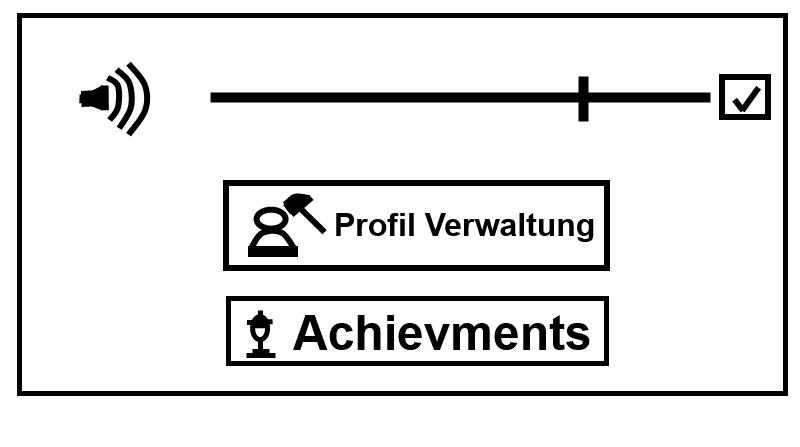
\includegraphics[width=\textwidth]{assets/Einstellungen}
	\end{minipage}

	\begin{minipage}{1\textwidth}
		\item \subsection*{Profilbearbeitungsmenü:}
		Dieses Menü ist identisch mit dem Menü zum Anlegen eines neuen Spielerprofils.\\
		Beendet man dieses Menü kommt man automatisch zurück ins Einstellungsmenü.\\
		Außerdem kann hier ein bestehendes Profil gelöscht werden. Sollte man ein Profil löschen, so landet man anschließend im Profilmenü um ein anderes Profil zu wählen.
		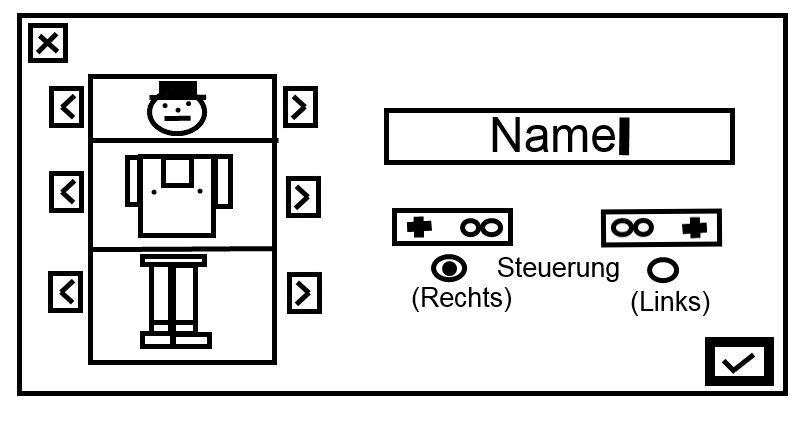
\includegraphics[width=\textwidth]{assets/CreateProfile2}
	\end{minipage}

	\begin{minipage}{1\textwidth}
		\item \subsection*{Achievements:}
		Hier sind alle Achievements zu sehen. Schon erreichte sind durch ein Bild gekennzeichnet, ansonsten ist dort ein Platzhalter zu sehen. Ein Abbruch führt zurück in die Einstellungen.\\
		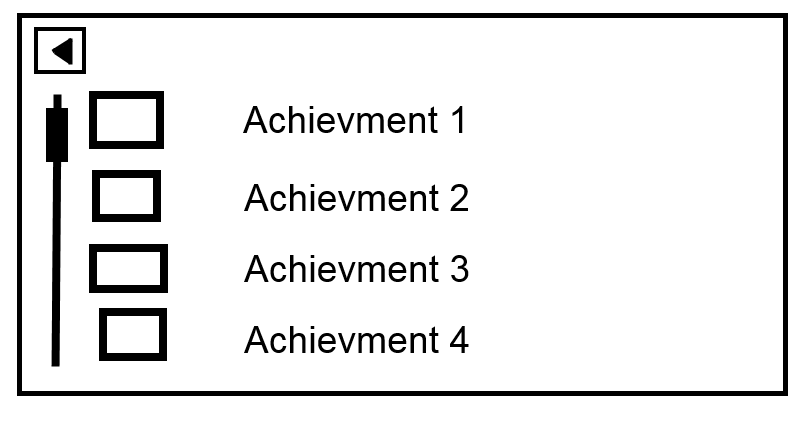
\includegraphics[width=\textwidth]{assets/Achievments}
		
	\end{minipage}
	
	\begin{minipage}{1\textwidth}
		\item \subsection*{Stageauswahl:}
		Hier kann man sich eine Stage zum spielen auswählen. Sie sind der Schwierigkeit nach geordnet und können im Spielverlauf freigeschaltet werden.\\
		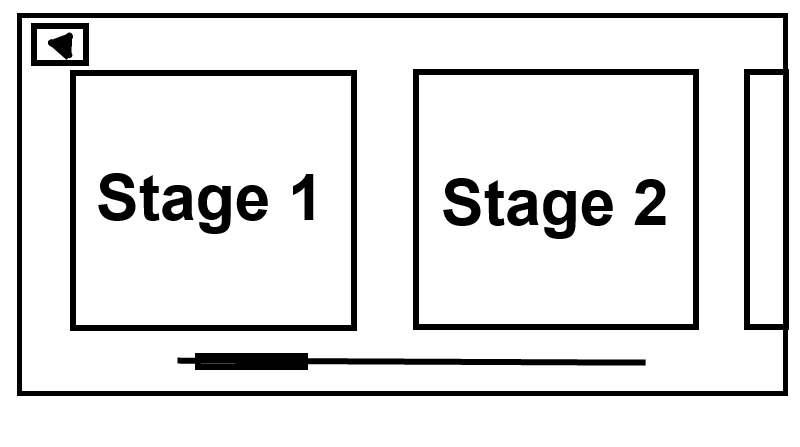
\includegraphics[width=\textwidth]{assets/Stagemenu}
	\end{minipage}
	
	\begin{minipage}{1\textwidth}
		\item \subsection*{Levelauswahl:} \label{appaufbau:Levelauswahl}
		Hier kann ein Level der Stage in der man sich aktuell befindet gestartet werden.(auch diese müssen nach und nach freigeschaltet werden).\\
		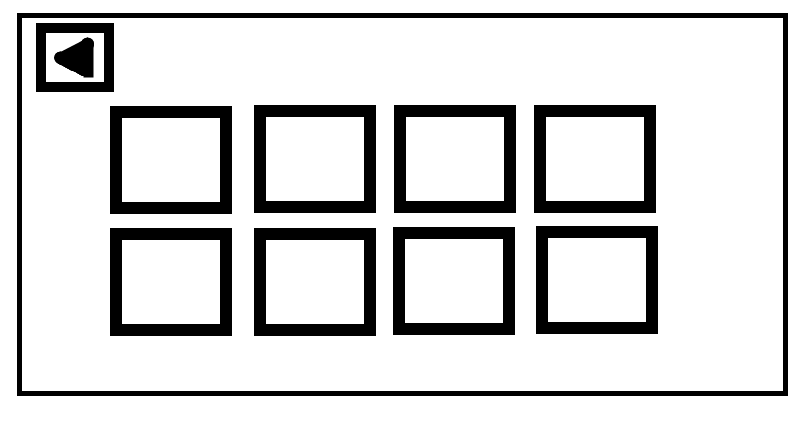
\includegraphics[width=\textwidth]{assets/Levelmenu}
	\end{minipage}
	
	\begin{minipage}{1\textwidth}
		\item \subsection*{Leveldesign:} \label{appaufbau:Leveldesign}
		Jedes Level  hat den selben Aufbau am unteren Rand sind die Button und das Steuerkreuz zum bedienen des Spielecharcters sowie ein Button um sich das aktuelle Level-ziel oder Hinweise zum Level geben zu lassen.\\ Die Anordnung der Buttons wird gespiegelt falls man als Linkshänder spielen will. Der komplette Buttonbereich ist transparent, sodass der Spieler mehr vom Spielfeld sieht.\\
		In der Linken Oberen Ecke ist ein Button der ins Levelmenü führt. Das Spiel wird dann pausiert und es erscheinen Buttons zum Neustart des Levels, dem verlassen ins Levelmenü, dem Verlassen ins Hauptmenü und Einstellungen(Lautstärke).\\
		Das eigentliche Spielfeld nimmt den Rest des Bildschirms ein.\\
		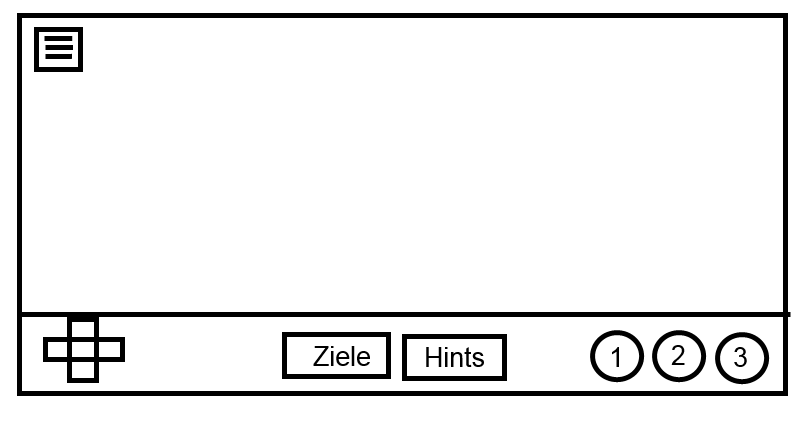
\includegraphics[width=\textwidth]{assets/LevelDesign2}
	\end{minipage}
	
	\begin{minipage}{1\textwidth}
		\item \subsection*{Auswertungsmenü:}
		Sollte der Spieler ein Level erfolgreich gelöst haben so kommt er ins Auswertungsmenü, hier werden ihm Informationen zu seinem Erfolg , sowie errungene Achievments mitgeteilt. Er hat die Wahl das nächste Level zu starten oder zurück zum Hauptmenü zu kommen. 
		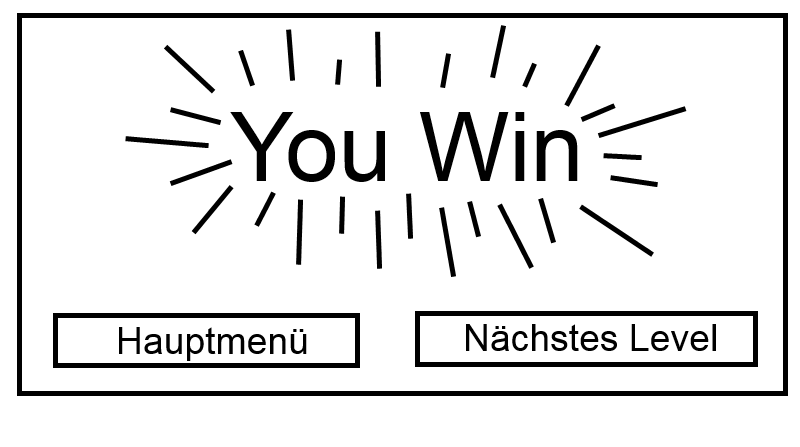
\includegraphics[width=\textwidth]{assets/Auswertungsmenu}
	\end{minipage}

\end{enumerate}

\clearpage

\begin{minipage}{1\textwidth}
\subsection{Appstruktur}
	Die folgende Grafik stellt die Struktur der App grafisch dar.\\
	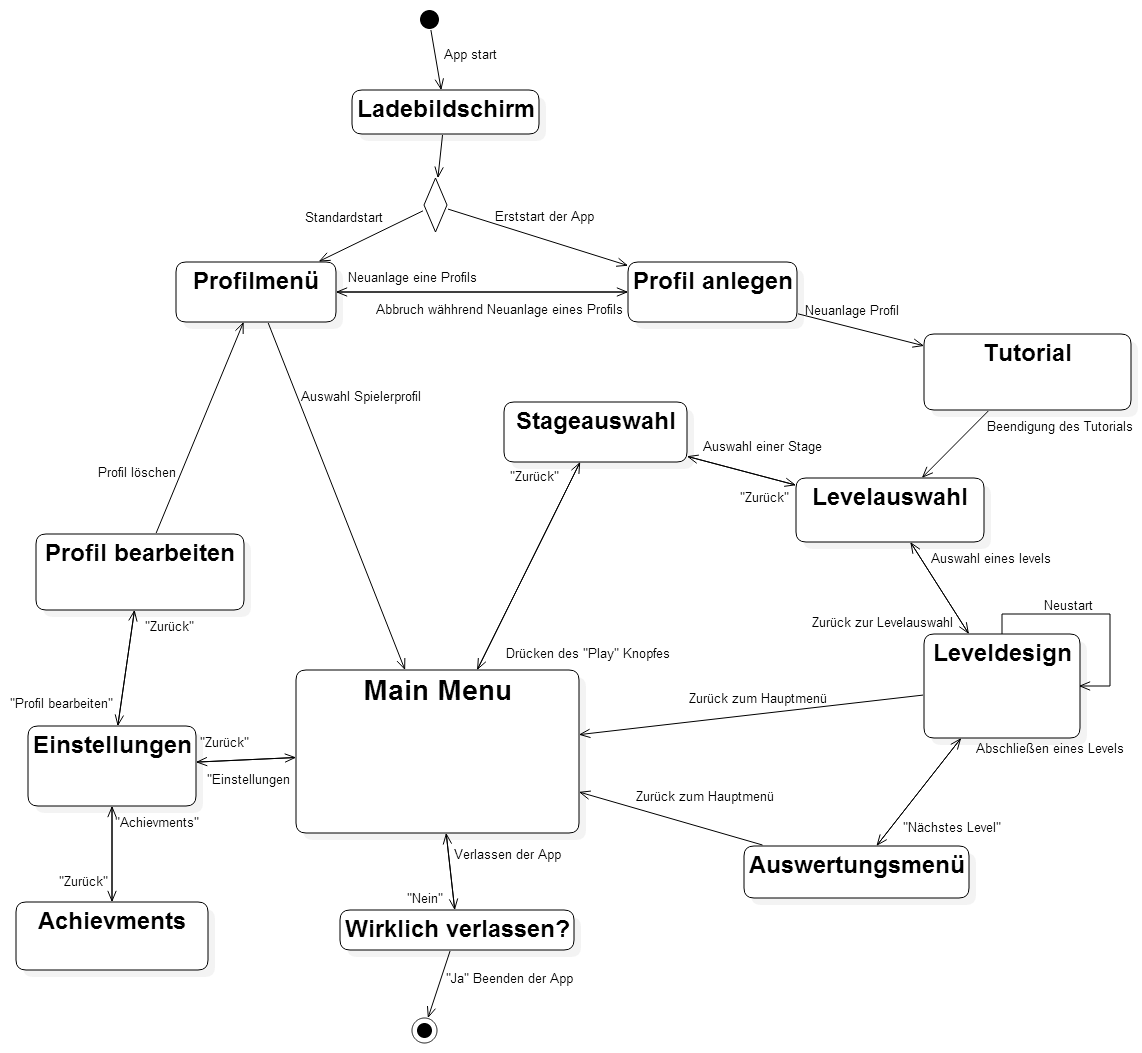
\includegraphics[width=\textwidth]{assets/Menustructur}
\end{minipage}

\begin{minipage}{1\textwidth}
\subsection{Benutzer Interaktionen}
Die folgende Grafik enthält die möglichkeiten des benutzers auf die App einzuwirken.\\
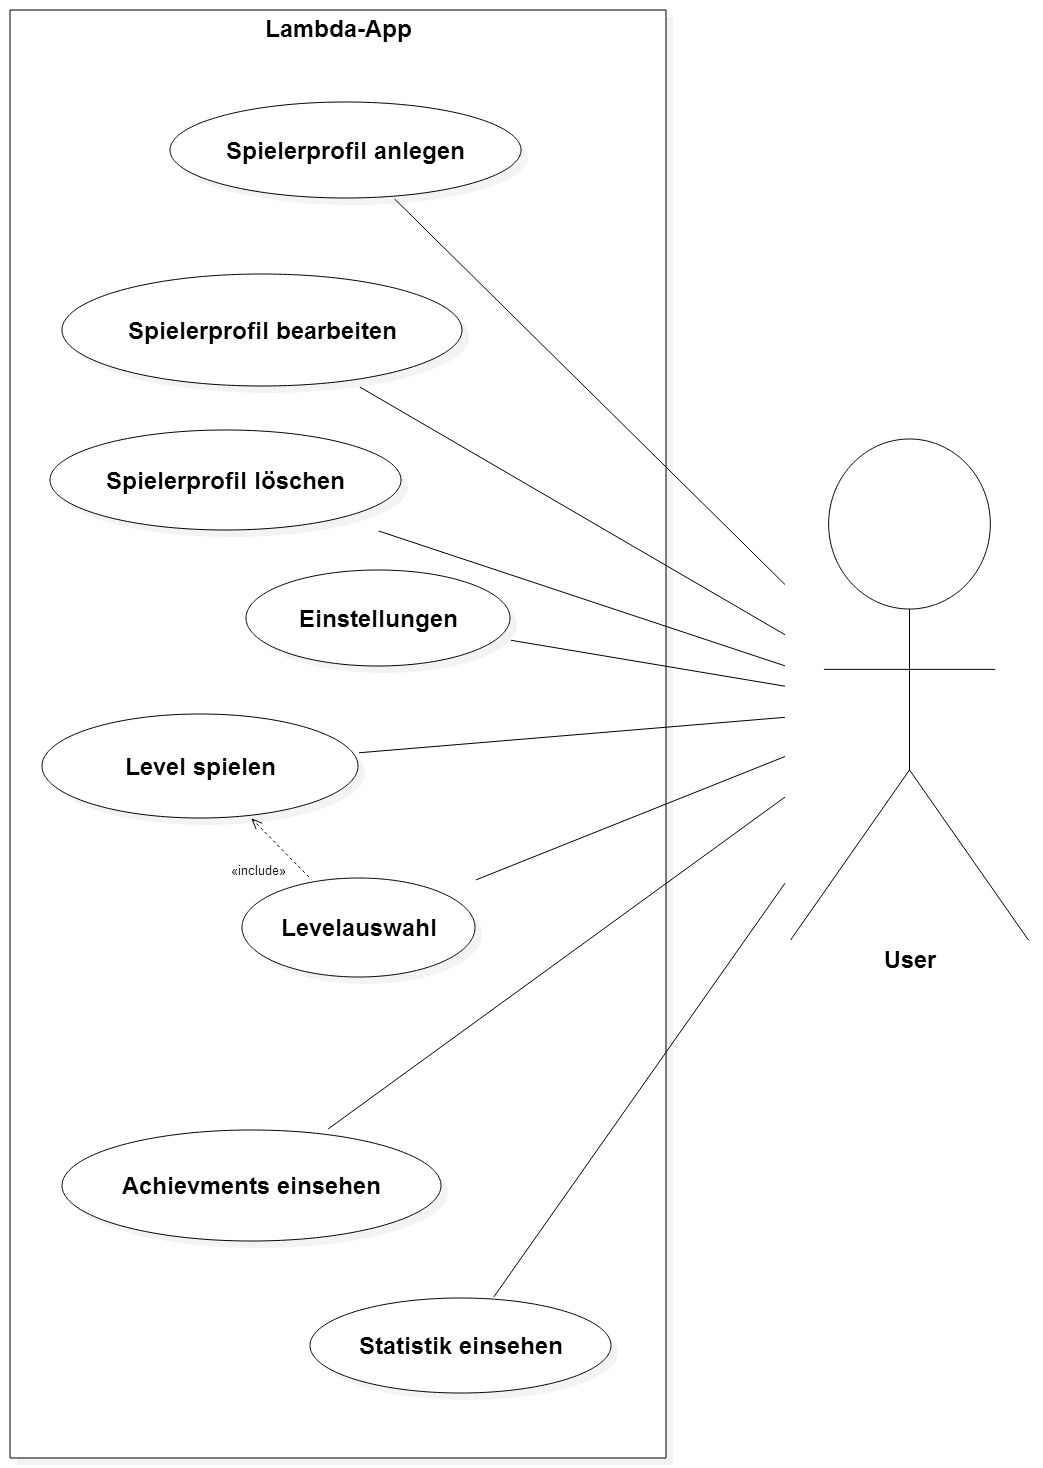
\includegraphics[width=\textwidth]{assets/Benutzerdiagramm}
\end{minipage}

\clearpage








% ---------------
% Szenarien
% ---------------
\section{Szenarien}

\subsection{Erstes Ausführen des Spieles} \label{szenarien:first_run}
	\begin{enumerate}
		\item Starten der Applikation durch Anklicken der App-Verknüpfung
		\item Der Ladebildschirm(\ref{appaufbau:Ladebildschirm}) wird sichtbar und informiert über den Ladezustand des Spieles.
		\item Der Spieler wird direkt zum "`Benutzer-Anlegen"'  weitergeleitet
		\item Wurde ein Benutzer angelegt, öffnet sich die Einstellung
		\item Geht der Spieler von den Einstellungen weiter, beginnt der Tutorial-Modus
		\item Lamdbalino begrüßt den Spieler
		\item Es wird in die Handlung des Spieles eingeführt
		\item Nach dem Tutorial-Modus öffnet sich das Levelmenü und das erste Level ist freigeschaltet 
	\end{enumerate}
	
\subsection{Benutzer-Profil anlegen} \label{szenarien:ProfilAnlegen}
	\begin{enumerate}
		\item \enquote{Benutzer-Profil anlegen} wurde gewählt
		\item Der Spieler wählt einen Avatar
		\item Er gibt seinen Namen an
		\item Er kann wählen, ob er Rechtshänder oder Linkshänder ist
		\item Mit dem \enquote{Menü}-Knopf kommt der Benutzer ins Hauptmenü (\ref{appaufbau:Hauptmenü})
	\end{enumerate}	
	
\subsection{Tutorial-Modus} \label{szenarien:tutorial_mode}
	\begin{enumerate}
		\item Das Auswählen des Levels wird animiert
		\item Die Elemente des Spieles werden erklärt
		\item Ein Level wird Schrittweise simuliert
		\item Es öffnen sich kleine Felder um die nächste Handlung animiert zu erklären
		\item Schließt man die Felder, geht das Tutorial weiter
		\item Wie die Level, wird gezeigt wie die Maschinen funktionieren und wie sie angeordnet werden müssen
	\end{enumerate}
	
\subsection{Allgemeiner Spielstart} \label{szenarien:allg_spielstart}
	\begin{enumerate}
		\item Starten der Applikation durch Anklicken der App-Verknüpfung
		\item Der Ladebildschirm(\ref{appaufbau:Ladebildschirm}) wird sichtbar und informiert über den Ladezustand des Spieles
		\item Nach dem Laden kann man den Benutzer aus vorhandenen Profilen auswählen oder man legt ein neues Profil (\ref{szenarien:ProfilAnlegen}) an
		\item Das Hauptmenü (\ref{appaufbau:Hauptmenü}) wird geöffnet		
	\end{enumerate}
	
\subsection{Spielen} \label{szenarien:spielen}
	\begin{enumerate}
		\item Im Hauptmenü wählt man die Stages
		\item In den Stages wählt man das Level (\ref{appaufbau:Leveldesign})
		\item Nach dem Öffnen des Levels, wird angezeigt, was die Maschine(n) produzieren müssen
		\item Möchte der Spieler erneut das gewünschte Produkt ansehen, kann er dies durch einen Knopf wählen
		\item Er spielt nach den Spielregeln (\ref{spielaufbau:Spielregeln})
	\end{enumerate}
	
\subsection{Einstellungen} \label{szenarien:einstellungen}
	\begin{enumerate}
		\item Im Hauptmenü wählt man den Punkt \enquote{Einstellungen}
		\item Dort kann man mithilfe eines stufenlosen Reglers die Lautstärke einstellen sowie den Button \enquote{Profil bearbeiten} (\ref{szenarien:ProfilBearbeiten}) drücken
		\item Über die \enquote{Zurück}-Taste des Geräts gelangt man in das Hauptmenü (\ref{appaufbau:Hauptmenü})
	\end{enumerate}

\subsection{Benutzer-Profil bearbeiten} \label{szenarien:ProfilBearbeiten}
	\begin{enumerate}
		\item Im Hauptmenü wählt man den Punkt \enquote{Einstellungen}
		\item Dort drückt man auf den Button \enquote{Profil bearbeiten}
		\item Hier kann man, wie schon beim Anlegen des Profils (\ref{szenarien:ProfilAnlegen}), den ausgewählten Avatar, seinen Namen und auch, ob Rechts- oder Linkshändersteuerung gewünscht wird, editieren.
	\end{enumerate}
	
\subsection{Benutzer-Profil löschen} \label{szenarien:ProfilLoeschen}
\begin{enumerate}
	\item Im Hauptmenü wählt man den Punkt \enquote{Einstellungen}
	\item Dort drückt man auf den Button \enquote{Profil bearbeiten}
	\item Durch drücken des Button \enquote{Profil löschen} erscheint dort ein Frage Fenster ob man das Profil wirklich löschen will.
	\item Mit einem Klick auf \enquote{Ja} wird das aktuelle Profil gelöscht, sofern noch mindestens ein anderes Profil existiert.
	\item Nach erfolgreichem löschen des Profils landet man automatisch im Profilmenü.
\end{enumerate}

\subsection{Informationen aufrufen} \label{szenarien:infomartionen_aufrufen}
\begin{enumerate}
	\item Im Hauptmenü wählt man den Punkt \enquote{Einstellungen}
	\item Dort klickt man auf den Button \enquote{Infos}.
	\item Es erscheint ein vereinfachte Erklärung des Lambda-Kalküls, sowie ein Erläuterung zu den Zusammenhängen des Lambda-Kalküls und des Spiels.
\end{enumerate}

\subsection{Statistiken} \label{szenarien:statistik}
	\begin{enumerate}
		\item Im Hauptmenü wählt man den Punkt \enquote{Statistiken}
		\item Dort können sowohl die Achievements, sowie verschiedene Statistiken zu Spieldauer etc. eingesehen werden.
	\end{enumerate}

\subsection{Achievements} \label{szenarien:achievements}
 \begin{enumerate}
 	\item Freischalten
 		\begin{enumerate}
 			\item Achievments werden während des spielen eines Level freigeschaltet
 			\item Über neu freigeschaltete Achievments wird der Spieler nach Abschluss eines Levels im Auswertungsmenü informiert
 		\end{enumerate}
 	\item Anzeige
 	 	\begin{enumerate}
 	 		\item Im Hauptmenü wählt man den Punkt \enquote{Einstellungen}
 	 		\item Dort wählt man \enquote{Achievments}
 	 		\item Es wird eine Liste aller Achievements angezeigt.
 	 		\item Freigespielte Achievements sind farbig markiert. 
 		\end{enumerate}
 \end{enumerate}

\subsection{Spiel verlassen} \label{szenarien:quit_game}
	\begin{enumerate}
		\item Spiel beenden
			\begin{enumerate}
				\item Man klickt auf den Button links oben im Hauptmenü
				\item Es erscheint ein Fenster \enquote{Wirklich verlassen?}
				\item Beim betätigen des Button \enquote{Ja} wird das Spiel verlassen und die App beendet
				\item Außerdem werden alle nicht gespeicherten Änderungen gespeichert
			\end{enumerate}
		\item Spiel über das Betriebssystem verlassen
			\begin{enumerate}
				\item Der Benutzer berührt den Homebutton auf seinem Gerät zum zurück zu Android zu gelangen.
			\end{enumerate}
	\end{enumerate}


\end{document}